\documentclass[preprint,12pt,authoryear]{elsarticle}     
\usepackage{amssymb}
\usepackage{graphicx}
\usepackage{amsmath}
\usepackage{mathptmx}  
\usepackage{subfigure}    % use Times fonts if available on your TeX system
%\usepackage{natbib}
\usepackage{tabularx}
\usepackage{hyperref}
\usepackage{lineno}

\journal{Cortex} 

\begin{document}

\begin{frontmatter}


\title{Bayesian multi-level modelling for predicting single and double feature visual search}

\author[inst1]{Anna E. Hughes}
\author[2]{Anna Nowakowska}
\author[1]{Alasdair D. F. Clarke}

\address[inst1]{Department of Psychology,%Department and Organization
            University of Essex, 
            Colchester,
            CO4 3SQ,
            UK}

\address[2]{School of Psychology,%Department and Organization
            University of Aberdeen, 
            Aberdeen,
            AB24 3FX,            
            UK}

\begin{abstract}
Performance in visual search tasks is frequently summarised by ``search slopes'' - the additional cost in reaction time for each additional distractor. While search tasks with a shallow search slopes are termed efficient (pop-out, parallel, feature), there is no clear dichotomy between efficient and inefficient (serial, conjunction) search. Indeed, a range of search slopes are observed in empirical data. The Target Contrast Signal (TCS) Theory is a rare example of quantitative model that attempts to predict search slopes for efficient visual search. One study using the TCS framework has shown that the search slope in a double-feature search (where the target differs in both colour and shape from the distractors) can be estimated from the slopes of the associated single-feature searches. This estimation is done using a contrast combination model, and a collinear contrast integration model was shown to outperform other options. In our work, we extend TCS to a Bayesian multi-level framework. We investigate modelling using normal and shifted-lognormal distributions, and show that the latter allows for a better fit to previously published data. We propose running a new fully within-subjects experiment to attempt to replicate the key original findings, with some changes to help distinguish between theories. 
\end{abstract}


\begin{keyword}
Visual search \sep  Efficient search \sep Parallel processing
\end{keyword}

\end{frontmatter}

\linenumbers

\section{Introduction}
\label{intro}

Visual search, where participants are asked to find a target within a cluttered scene, has been extensively studied within psychology. Several models have been developed that can generate testable predictions about how different types of distractors and targets affect search efficiency. One of the key distinctions in the field has been between efficient (also referred to as parallel or pop-out) and inefficient (serial) search. These are often studied in the context of the regression slope between the number of distractors and mean reaction time, which has been termed the \textit{search slope}. When the search slope is shallow (usually positive, but occasionally negative e.g. \citep{rangelov2017failure}), the search is called efficient or parallel, and the addition of more non-target distractors has little impact on an observers difficulty in finding a target. When the slope is steeper, each additional distractor has a noticeable impact on increasing difficulty, and the search is described as inefficient or serial. However, the distinction between these types of search is often less clear in real experimental data, with a range of different search slopes being seen for different types of targets and distractors \citep{duncan1989visual,cave1990modeling,wolfe1998can,liesefeld2016search}. Recent work has also attempted to model the variation in search slopes at the boundary between inefficient and efficient search \citep{liesefeld2016search}.

In the current study, we are interested in what has traditionally been termed efficient or parallel search, and the factors that affect search slope in these conditions. Recent work has suggested that for efficient search, there is a logarithmic relationship between distractor set size and reaction time, and that this relationship can be modified by target-distractor similarity \citep{buetti2016towards}, providing evidence that search behaviour in parallel search is more complex than has previously been assumed. This observation has formed the basis of the `Target Contrast Signal (TCS) Theory' \citep{lleras2020target}, which aims to provide a means of predicting observer search slopes for new search arrays by quantifying target-distractor differences. For example, by measuring search slopes for conditions in which the distractors differ from the target along a \textit{single feature} (e.g. colour \textit{or} shape), it has been shown that you can predict search times for arrays in which the target differs from the distractors along two features (e.g., colour \textit{and} shape) which we refer to here as \textit{double feature} search \citep{buetti2019predicting} (but similar paradigms have been known by other names e.g. 'redundant feature search' \citep{krummenacher2012dynamic, mordkoff1991interactive}). Here, we aim to replicate and extend this work both theoretically and empirically, to test the generalisability of the TCS model, and to suggest ways in which the TCS model could be modified to generate better predictions.

\subsection{Previous Work}

Many different forms of visual search models have been proposed. One well developed class of models are the saliency models, which aim to predict eye movements during scene viewing, including visual search. They rest on the assumption that fixations are directed to objects or locations that are most dissimilar to the background or other objects in the visual display \citep{itti2000saliency, itti1998model, koch1987shifts}. While the original saliency model was able to predict fixation allocation in a visual search task above chance \citep{parkhurst2002modeling}, further research demonstrated that a comparable level of performance could be achieved using a simple central fixation bias heuristic \citep{tatler2007central}. The saliency models have since been extended and improved (see for example \cite{zhang2008sun}): however, the main issue with this family of models remains their limited usability in complex real-life search arrays \citep{tatler2011eye, koehler2014saliency}, and even in abstract laboratory search arrays \citep{kotseruba2020saliency}. In addition, in most instances of visual search, the target is clearly defined (i.e. the goal is to find a specific object) and inspecting the most salient areas of the display may in these cases be inefficient. Finally, by focusing on eye movements, these models do not necessarily provide a theoretical framework for the cognitive processes underlying visual search.

Perhaps the most established class of models of visual search are based around Feature Integration Theory \citep{treisman1980feature}, which has been modified and extended by Wolfe and colleagues in the Guided Search Model \citep{wolfe1989guided,wolfe2014approaches}. These theories have been developed using data from visual search tasks with discrete sets of abstract items. These models combine top-down influences (how closely an item resembles the observer's goal) with bottom-up image properties. For example, if one's goal (top-down processing) is to find a red horizontal bar, all the red and horizontal items in a visual search display will be given greater weight than distractors (e.g. vertical and blue items) in the model. The salience of a given object in the display (how distinctive it is from the surrounding objects) also activates bottom-up processing. For instance, a blue item among red items is ranked higher than red among orange items. In such cases, a salient item can capture attention even without resembling the target. Combining bottom-up and top-down sources of activation generates an activation map which generates a prediction of the order in which stimuli are processed in visual search. Other extensions to these models have been proposed, such as the Dimension Weighting Account, in which saliency weightings are assigned to different target 'dimensions' (e.g. colour or shape), helping to explain results where varying the target dimension within blocks of trials leads to longer reaction times than where the dimension remains consistent within a block \citep{krummenacher2012dynamic}. Thus, these models aim to produce a representation of the visual properties of the distractors at each location in the visual field. However, these are predominantly qualitative models, and thus it is difficult to use them to make specific quantitative predictions. 

TCS falls under a class of models that take a different approach, in that they focus solely on representing the difference between targets and distractors. For example, in work on eye movement patterns, it has been proposed that performance in inefficient (serial) visual search is mostly determined by the size of the `functional viewing field', whose size varies as a function of target-distractor similarity \citep{hulleman2017brink}. Similarly, work on attention has proposed the notion of `relative features', where attention is tuned to feature relationships i.e. the appearance of the target relative to distractors in the environment \citep{becker2014color, becker2010role}. TCS also has features in common with other models that propose parallel identification of all items in a scene, with diffusion based mechanisms for identifying targets from distractors \citep{moran2013competitive, moran2016serial}. However, TCS \citep{lleras2020target} aims to provide a unifying framework that can make quantitative behavioural predictions for visual search based on this general assumption. As such, it is an attractive candidate model for a formal registered replication.

A key assumption of the TCS model is that behaviour is determined by comparing the target template (held in memory) with every element present in the scene in parallel. This allows the visual system to reject peripheral non-targets quickly; the speed at which items are evaluated is determined by how different the item is from the template through an evidence accumulation process (formally, the slope of the logarithmic function is assumed to be inversely proportional to the overall magnitude of the contrast signal between the target and distractor). The model thus focuses on an initial, efficient processing stage of search; if sufficient evidence is not accumulated during this process, the model posits that a second stage is entered, requiring a sequence of eye movements to search for the target in a serial manner. TCS has been successful in predicting a number of empirical results, including search performance in heterogeneous scenes based on parameters estimated in homogeneous scenes, both with artificial stimuli \citep{buetti2016towards,lleras2019predicting} and with real-world objects visualised on a computer display \citep{wang2017predicting}. Table \ref{tab:tcs_overview} provides an overview of studies investigating the TCS framework to date.
 
The original version of the TCS model is essentially a (natural) log-linear model in the number of distractors. The full model contains a variable $L$, which represents the number of different types of distractors present in the display. However, in our paper, we will follow \cite{buetti2019predicting} and only consider the specific case of $L=1$, of a target among a homogeneous set of distractors. In this case, the TCS model can be represented in the following way:


\begin{equation}
\hat{RT} = a + D\log(N_T+1)
\label{eq:loglin}
\end{equation}

The intercept, $a$, corresponds to search arrays in which only the target is present and there are no distractors. $N_T$ is the total number of distractors.

\begin{table}[hp]
\centering
\begin{tabularx}{\textwidth}{lX}
Reference & Overview\\
 \hline 
\cite{buetti2016towards} & For efficient search with a specific target, there is a logarithmic relationship between distractor set size and reaction time. The steepness of this relationship is modulated by distractor-target similarity, with steeper slopes for more similar distractors.\\
\cite{wang2017predicting} & Data from homogeneous search arrays can be used to predict search reaction times in heterogeneous displays containing images of real-world objects, using an equation assuming parallel, unlimited capacity, exhaustive processing, and independence of inter-item processing. \\ 
\cite{madison2018role} & Logarithmic efficiency in efficient search cannot be explained by crowding in peripheral vision. \\
\cite{ng2018fixed} & Logarithmic efficiency in efficient search cannot be explained by eye movements. \\
\cite{lleras2019predicting} & Validation of previous results showing data from homogeneous search arrays can be used to predict reaction times in heterogeneous displays. Distractor-distractor interactions can also facilitate processing when nearby items are similar to each other. \\
\textbf{\cite{buetti2019predicting}} & Data from search arrays where the distractors are distinguished from the target by one feature can be used to predict search reaction times in displays with compound stimuli, defined by two features. Reaction times can be predicted using a collinear contrast integration model, which assumes that the overall target-distractor contrast is the sum of the contrasts from the two feature vectors separately. \\
\cite{lleras2020target} & Full proposal of the Target Contrast Signal Theory, proposing that the initial stage of processing computes a difference signal between each item in the scene and the target template, using this to determine which items in the scene are unlikely to be the target. \\
\cite{ng2020prioritization} & Attention works in a two stage process, first discarding target-dissimilar distractors in a distributed, parallel way. Focused spatial attention then visits target-similar items at random. \\
\cite{xu2021predicting} & Extension of \cite{buetti2019predicting} to new features (shape and texture), which combine according to a Euclidean metric (orthogonal contrast integration model). \\
\end{tabularx}
\caption{An overview of work on the Target Contrast Signal Theory. The key paper for our replication is highlighted.}
\label{tab:tcs_overview}
\end{table}

\subsection{Rationale for proposed work}

While many aspects of the TCS framework have been tested, with extremely promising results, there remains a great deal of scope for verification of some of the key findings to date, and extensions of aspects of the model. In all implementations of TCS so far, predictions of search efficiency (e.g. in heterogeneous scenes) have been made on the average of a group of participants, using data from a different group performing a different task (e.g. searching in homogeneous scenes). Thus, we know that TCS can replicate group-level averages between subjects in search well, but we do not know to what extent it is also able to make predictions at the individual level. This is particularly important given that conclusions based on aggregate data can be different from those that take individual differences into account; in one study where participants searched for a target in an array of randomly oriented line segments, aggregating the data suggested that participants were using a stochastic search model \citep{nowakowska2017human}. However, when considering each participant individually, it became clear that there was a high level of heterogeneity in responses, with some participants performing close to optimally, and others actually performing worse than chance \citep{nowakowska2017human}. Similarly striking variability has also been reported in other search studies \citep{irons2016choosing, irons2018characterizing, clarke2020stable}. 

Taking search time distributions into account is also important for constraining theories of visual search \citep{wolfe2010reaction, liesefeld2020theoretical}: for example, they have been used to help distinguish between models that make similar predictions at the level of average reaction times \citep{moran2016serial, moran2017appeal}. Including subject and trial level data into our implementation of the TCS will therefore further aid model development and assumption testing.

We also extend the TCS model into a Bayesian framework, where we begin with existing 'prior' beliefs that are updated with data to give 'posterior' beliefs that can be used for inference \citep{mcelreath2020statistical}. We think this has a number of advantages over frequentist approaches. Perhaps most importantly, Bayesian models are highly flexible. We demonstrate how we are able to specify a model that is able to more accurately represent the distribution of responses (for example, by specifying a response distribution that avoids predicting negative reaction times) with a relatively complex model structure, that can be fit to a relatively small amount of pilot data: something that would be challenging within a frequentist framework. We also believe that Bayesian models offer very intuitive methods for model testing and comparison and straightforward interpretation of results, and we hope that this manuscript can act as a demonstration of these benefits, showing how they can be applied to real scientific questions beyond the simplified examples often found in textbooks or tutorials.

In the current manuscript, we focus on replicating and extending findings from \cite{buetti2019predicting}. In their study, participants searched for a target in a scene of homogeneous distractors (see Figure \ref{fig:buetti2019_stimulus}). First, parallel search efficiency (measured by the logarithmic search slope) was estimated for cases where the distractors varied from the target in one dimension: either colour (e.g. a cyan target being searched for in either yellow, blue or orange distractors) or shape (e.g. a semicircle target in either circle, diamond or triangle distractors). New participants then searched for the same targets in displays where the distractors were compounds, differing from the target in both colour and shape (e.g. searching for a cyan semicircle in either blue circles, orange diamonds or yellow triangles). The logarithmic search slopes in the initial experiments were then used to predict the logarithmic slopes and reaction times using a number of models. The authors found that the best model was a `collinear contrast integration model' where the distinctiveness scores were summed along each attribute in the unidimensional experiments, creating an overall contrast score that was used for compound stimuli predictions. In our registered replication, we will attempt to verify the conclusions of \cite{buetti2019predicting}, that the collinear contrast integration model does indeed offer the best characterisation of contrast signal combinations in visual search within the TCS framework.

\begin{figure}[ht]
\centering
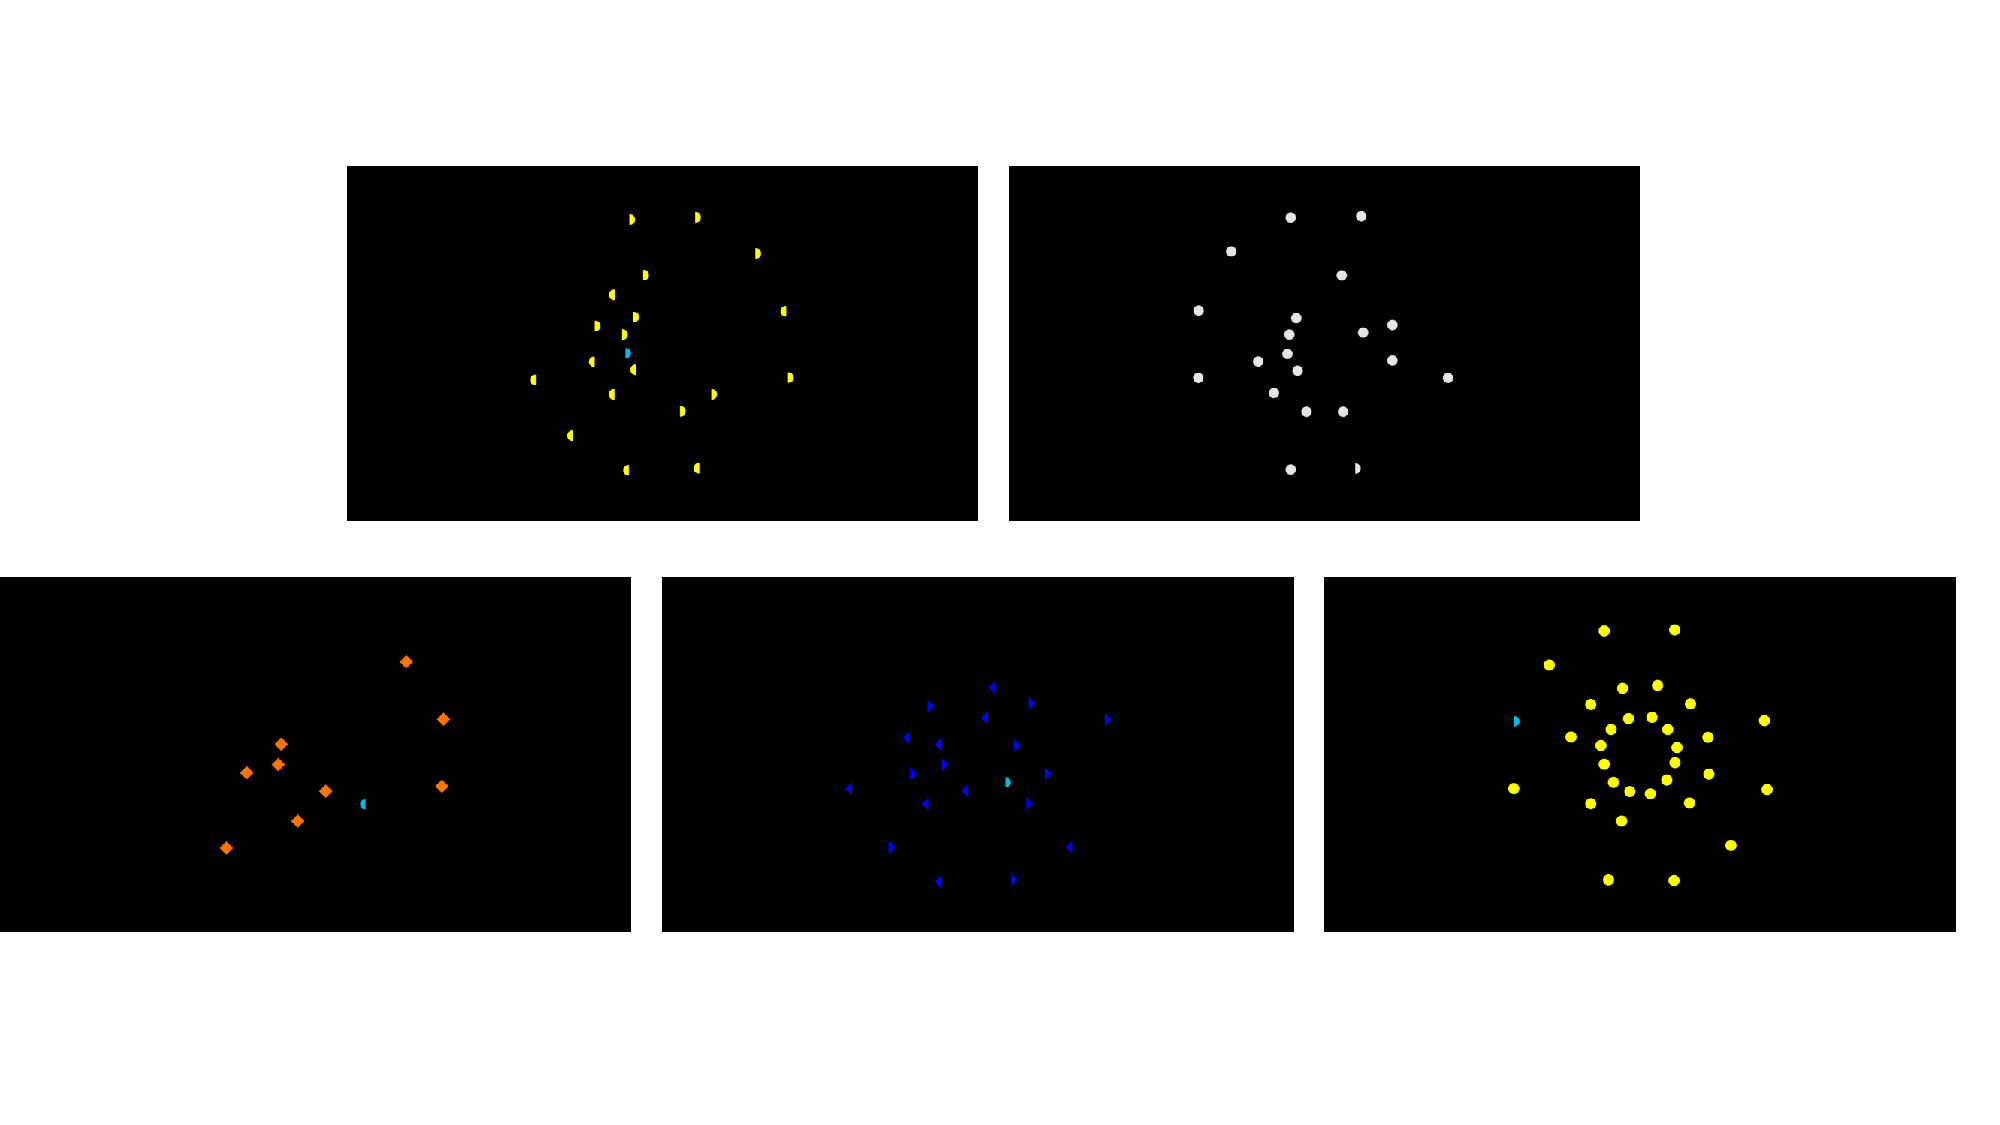
\includegraphics[width=\textwidth]{../plots/example_stimuli_figure.pdf}
\caption{Example stimuli from \cite{buetti2019predicting} Top left: Expt 1A. Here, the target is a blue semicircle within a set of homogeneous (yellow semicircle) distractors. Top right: Expt 1B. The target is a grey semicircle in circular grey distractors. Bottom left: Expt 2A. The target is a blue semicircle in orange diamond distractors. Bottom middle: Expt 2B. The target is a blue semicircle in dark blue triangle distractors. Bottom right: Expt 2C. The target is a blue semicircle in yellow circular distractors.}
\label{fig:buetti2019_stimulus}
\end{figure}

We begin by verifying the analysis of \cite{buetti2019predicting}. We then describe our proposed replication study, showing with pilot data how we are able to extend their model of how multi-dimensional contrasts are calculated, both by incorporating a multi-level design to predict within-subjects effects and by utilising a Bayesian generalised linear model framework to better represent the distribution of responses (e.g. avoiding predicting negative reaction times, accounting for uncertainty in model predictions). 

\section{The Target Contrast Model}
\label{sec:reansalysis}

We first describe the original Target Contrast Model, as presented in \cite{buetti2019predicting} and verify that we can succesfully replicate the original analysis (both using frequentist modelling and Bayesian modelling; see \textit{Supplementary Materials)}.

\subsection{TCS modelling overview} 

In Experiment 1a of \cite{buetti2019predicting}, participants searched for a cyan semicircle target among blue, yellow or orange semicircular distractors i.e. they searched for a target that differed from the distractors by a \textit{single feature} (colour). The experiment was then repeated (1b) using a different single feature (shape, with participants searching for the semicircular target within triangle, circle or diamond distractors). In Experiments 2a, 2b and 2c, participants again searched for a cyan semicircle, but this time, the distractors differed in both shape and colour. We will refer to these conditions as \textit{double features}. Note, unlike in standard conjunction searches, in this paradigm, the distractors are all identical with respect to these features (i.e, orange triangles). Examples of all these stimuli are shown in Figure \ref{fig:buetti2019_stimulus}. \cite{buetti2019predicting} also carried out a replication of their basic results using slightly different target and distractor stimuli (Experiments 3 and 4).

The \textit{Target Signal Contrast} theory is built around a linear model for predicting mean reaction times from the logarithm of the number of distractors (see Equation \ref{eq:loglin}). In particular, the TCS theory allows us to predict the value of the logarithmic slope, $D_\text{c,s}$, in this condition based on the corresponding $D_i$ in the single feature search experiments. 

\subsubsection{Calculating the intercept, $a$, and the logarithmic slope parameter, $D_i$}
\label{sec:fitting_D}

Experiments 1a and 1b and 3a and 3b were used to calculate the logarithmic slope parameter $D_i$. In all experiments, the number of distractors varied, allowing the data to be used to fit a log-linear model for reaction times, where reaction times increase logarithmically with $N_T$, the number of distractors (see Equation \ref{eq:loglin}). In the original model the error distribution was assumed to be normal. Thus the results of Experiments 1 and 3 were used to calculate $D_i$, for each type of distractor. When colour varied, we will refer to $D_c$, for $c=1,2,3$. Similarly for shape we will denote this ($D_s$), and the compound features are denoted as ($D_{c,s}$). 

Fitting the model specified in Equation \ref{eq:loglin} to the data, we obtain the values for $D_c$ and $D_s$ given in Table \ref{tab:reimp_Dc_Ds}. As can be seen, the more similar the distractors are to the target, the steeper the slope parameter is. 

\begin{table}[h]
\centering
\begin{tabular}{ c|c||c|ccc } 
feature & $D_c$ & feature & $D_s$\\
 \hline 
blue & 76.8 & triangle & 141.1\\
yellow & 16.0 & diamond & 77.2\\
orange & 9.8  & circle & 62.1\\
\end{tabular}
\caption{A table of $D_i$ values for Experiment 1a and 1b. See \textit{Supplementary Materials} for full values for all experiments.}
\label{tab:reimp_Dc_Ds}
\end{table}

\subsubsection{Estimating $D_{c,s}$, the logarithmic slope parameter for compound features}

In the context of the current experiments, the core idea of TCS theory is that we can estimate the (natural) logarithmic slope parameter for a double feature visual search from the slopes parameters in the two independent single feature searches i.e., $D_{c,s} = f(D_c, D_s)$. \cite{buetti2019predicting} tested three different models for predicting $D$ for compound colour-shape stimuli. The best feature guidance model (Equation \ref{eq:bestfeature}) suggests that when the target and lures differ in two dimensions, participants will choose to attend to whichever feature dimension is the most discriminable (i.e. has the smallest $D$ value):

\begin{equation}
D_\text{c,s} = \text{min}\left(D_\text{c}, D_\text{s}\right)
\label{eq:bestfeature}
\end{equation}

The orthogonal contrast combination model instead suggests that independent feature dimensions comprise a multidimensional space, where an object can be described by the overall vector in this space, and thus $\mathrm{D_{c,s}}$ can be represented as:

\begin{equation}
D_\text{c,s} = \frac{1}{\sqrt{{(\frac{1}{D_\text{c}}})^2 + (\frac{1}{D_\text{s}})^2}}
\label{eq:orthogonalcontrast}
\end{equation}

Finally, the collinear contrast integration model also assumes independence of feature dimensions, but assumes that while the visual features create a multidimensional space, the contrast between them is unidimensional. As $D$ is assumed to be inversely proportional to contrast, the equation can be written as follows:

\begin{equation}
\frac{1}{D_\text{c,s}} = \frac{1}{D_\text{c}} + \frac{1}{D_\text{s}}
\label{eq:collinearcontrast}
\end{equation}

\cite{buetti2019predicting} found that with their dataset, the collinear contrast integration model was best able to predict $D_{c,s}$ from $D_c$ and $D_s$, with $R^2 = 0.915$. We verified we were able to replicate this result using the dataset available on OSF (https://osf.io/f3m24/)\footnote{downloaded on 28th August 2020} and using the exclusion criteria originally applied; see Figure \ref{fig:comp_rep} (left panel) and \textit{Supplementary Materials} for details. We show that we are able to do this using both the frequentist modelling approaches used in the original paper, and using Bayesian modelling.

\begin{figure}
\centering
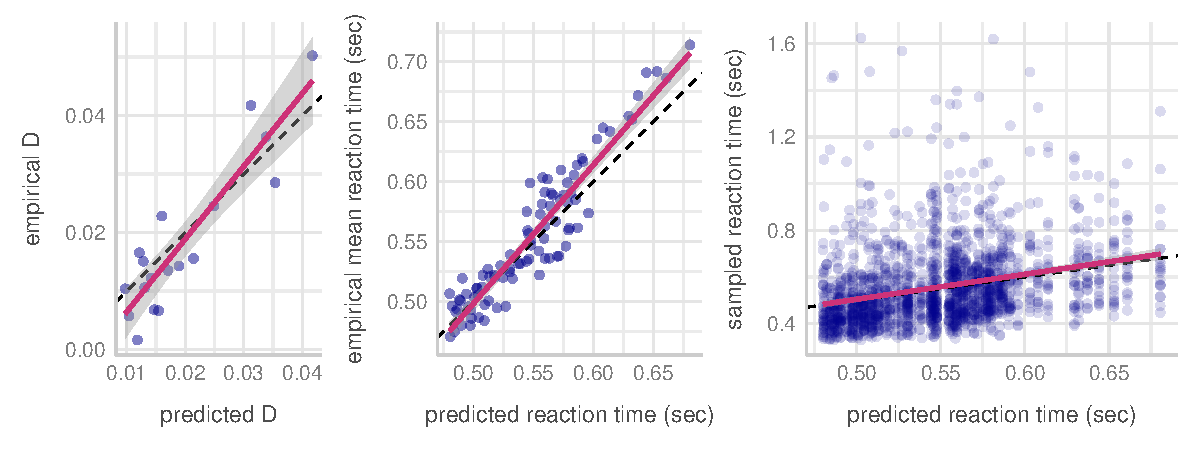
\includegraphics[width=\textwidth]{../plots/computational_replication.pdf}
\caption{(left) The collinear method for calculating $D$ offers a good prediction. (centre) Using the TCS to predict reaction times. (right) Each dot now represents a randomly sampled reaction time from an observer. Note that there is greater spread in the data points here, due to the fact that there will be trial-to-trial variability due to target position, inter-item distances, observer differences and so on.}
\label{fig:comp_rep}
\end{figure}

\subsubsection{Estimating $a$, the intercept parameter for compound features}

As $a$ is the intercept of the model, it represents how long observers take to find a target when $N_T = 0$, i.e., there are no distractors. As such, it should be independent of both shape and colour, and can be thought of as the role of non-search processes (such as motivation, motor preparation etc.) that influence reaction time. In \cite{buetti2019predicting}, $a$ was calculated for each sub-experiment. Here, we follow that method in order to replicate their results exactly. 

\subsubsection{Estimating mean reaction times}

Finally, we can use Equation \ref{eq:loglin} to predict mean reaction times. As can be seen in  Figure \ref{fig:comp_rep} (centre panel), these predictions are essentially identical to the empirical RT results: $R^2 = 0.93\%$.

\subsubsection{Discussion}

While TCS theory offers a good prediction of search slopes and corresponding mean reaction times for double feature search, there are two related limitations. Firstly, it is unable to account for individual differences between observers, only the changes to the sample average. Secondly, it cannot account for the distribution of reaction times over multiple trials. Figure \ref{fig:comp_rep} (right panel) shows clearly that these factors generate high levels of variability within the individual trial-level data. To address these issues, we propose adapting TCS to make use of multi-level modelling techniques. Multi-level models allow us to take into account the hierarchical structure of the data (i.e. that each participant completes multiple trials) in a way that does not require averaging, meaning that we are able to model participant variability as well as group-level effects \citep{gelman2006data}.

\subsection {A multi-level TCS}

Switching from a linear regression model to a multi-level model will allow us to compute $D$ for each participant, while simultaneously estimating the trial-to-trial variance. We also switch from a frequentist to Bayesian framework, as this allows us to naturally account for the uncertainty in the model’s predictions. However, switching from linear regression to a multi-level model raises the problem of which distribution to use for modelling reaction times. Using a normal distribution is unlikely to be satisfactory, as it is unable to account for the skew frequently seen in reaction time distributions, and also allows the possibility of negative reaction times. We can account for both of these problems by using a log-normal distribution. We will also test whether a slightly more complex extension of this model, the shifted lognormal model (which allows the distribution to be offset to the right i.e. mimicking the patterns seen in reaction time data, where valid responses begin at around 100ms) offers any improvement in model fit. Note that a Wald, or inverse Gaussian distribution, would also be a reasonable distribution choice for this data given that TCS is based on a diffusion process e.g. \citep{moran2013competitive}, and this distribution has been argued to be psychologically more plausible (e.g. \cite{kieffaber2006switch}, though see \cite{matzke2009psychological}): we chose not to use this distribution as it often leads to computational issues, which would make it harder for others to reproduce or build on our approach later.

\section{Hypotheses}

We plan an experiment to test the extent to which the original results in \cite{buetti2019predicting} replicate and generalise, using our new modelling approach.

\subsection{Proposed Modifications to Experimental Design}

In order to better test the above, and increases sensitivity, we propose to make the following changes to the experiment described in \cite{buetti2019predicting}:

\begin{enumerate}
\item \textbf{Within-subjects design.} This modification should give us greater power to detect differences between different models, as well as allowing us to investigate how individual differences in the single-feature task might explain differences in the double-feature task.
\\
\item \textbf{Increase target-distractor similarity.}  If the distractors are a very different colour from the target, they may not distinguish well between different contrast models. We will therefore run a version of the experiment where the target is a red semicircle, with distractors being either orange, purple or pink.
\\
\end{enumerate}

\subsection{Registered Hypotheses}

\begin{enumerate}
\item \textbf{Shifted lognormal model.} We hypothesise that a shifted lognormal model will give the best fit to our single-feature data, when compared to a lognormal and a normal model. \\
\item \textbf{Log-linear effect of $N_T$.} We will test the TCS model assumption that $N_T$ has a log-linear effect by testing models with and without the log of this term. We expect that this will confirm the results previously seen in papers testing TCS i.e. that the log-linear approach will be best.\\ 
\item \textbf{Contrast model comparisons.} We will test the hypothesis proposed by \citep{buetti2019predicting}: specifically, that the \textit{collinear contrast integration model} outperforms the \textit{best feature guidance}, and \textit{orthogonal contrast combination models} for the calculation of $D$, by calculating and comparing the mean absolute prediction error for each model. \\
\item \textbf{Reaction time predictions.} We will further test the hypothesis proposed by \citep{buetti2019predicting} by testing which model gives the best prediction at the trial-by-trial RT level.
\end{enumerate}

We will test each of these hypotheses by calculating the marginal likelihood of the relevant models, and then calculating the posterior probabilities. This will give us a probability for each model that represents the likelihood that the model gives the best prediction. We will consider there to be evidence for one model over the others if a given model has a probability above 90\%. We will consider there to be strong evidence for one model over the others if that model has a posterior probability above 99\%. This approach is most appropriate for our model: other measures of model fit, such as AIC, require an assumption of flat priors (which is not valid for multi-level models) and are based on point estimates (which is not valid for Bayesian models) \citep{mcelreath2020statistical}.

\subsection{Planned Explorations}

We plan to investigate the effect of individual differences in this paradigm: to what extent performance in the single-feature task can predict performance in the double-feature task for a given individual (\cite{buetti2019predicting} were not able to investigate this due to the between-subjects design of their study). We plan to do this by specifying a more complex random effects structure for the model, that allows for individual differences across different slopes for different features. This allows us to then study the random effect correlation structure. However, given these models can be challenging to fit, we will do this in an exploratory manner after carrying out our formally registered analysis.

One of the benefits of using a multi-level modelling approach is that it is relatively easy to extend to incorporate other factors that may contribute to reaction times, such as eccentricity and inter-item distance, which may help to explain behaviour further. To demonstrate this, we will also run exploratory analyses including a factor for which ring the target is in to assess whether this improves model fit or affects any of the conclusions that can be drawn from the model.

\subsection{Pilot Experiment}

Full details of a pilot experiment with $n=4$ participants (960 trials each) using our proposed analyses can be found in \textit{Supplementary Materials}. This suggests that even with a small sample, we can convincingly demonstrate H1 and H2. However, more data will be required to discriminate between the models, particularly for H4. Given that our methods are within-subject, we have reduced the number of trials per condition compared to \cite{buetti2019predicting} (12 in our pilot study, 20 in our proposed, compared to 40 in theirs). It is therefore possible that the increased noise in our estimated $D$ single-feature parameters will make it more difficult to predict double-feature $D$s accurately. However, we think this is unlikely to be the case as we can see that even in a small amount of pilot data, we can verify H3, with the collinear model having the lowest mean absolute prediction error.  

\section{General Methods}

\subsection{Sample Size: Participants and Trials}

We plan to test 40 participants during the experiment. Our pilot experiment shows that H1 and H2 are easily demonstrated with 10 times less data, and \cite{buetti2019predicting} used 20 participants per experiment. Our sample size will therefore be in line with previous work testing H3 and H4. 
Ethical approval for the study was granted by the University of Aberdeen (application number PEC/4677/2021/2).

Our pilot study above suggests that just 12 trials per condition may be sufficient to fit our models. To be conservative, we propose using 20 in our experiment. We have demonstrated that using just half the data (20/40 trials per condition) from \cite{buetti2019predicting} makes no difference to our computational verification (see \textit{Supplementary Materials}).

Finally, we have carried out a simulation experiment to estimate the confidence intervals on the mean when sampling from a log-normal distribution. We defined our distribution to have a mean-log of 6.135 and a standard deviation of 0.32. These values were loosely based on the distributions of reaction times in \cite{buetti2019predicting}. The results are shown in Figure \ref{fig:n_trials}. Based on these simulations, we find that a sample of $n=20$ leads to a 95\% confidence interval that is approximately 1.4 times larger than $n=40$. We feel this is a suitable compromise given we will be collecting our data within-subjects. 

\begin{figure}
\centering
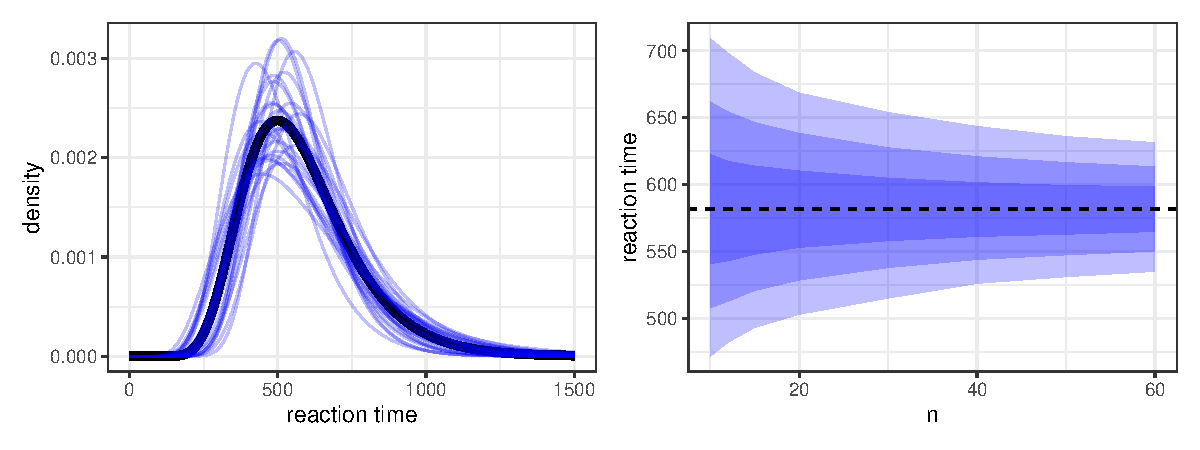
\includegraphics[width=\textwidth]{../plots/n_trials.pdf}
\caption{(left) The dark line shows the distribution we sampled from. The blue lines show distributions fitted to different samples of 20 data points. (right) Plot showing how the distribution of sample means vary with $n$. Shaded regions indicate the 50\%, 80\% and 95\% confidence intervals.}
\label{fig:n_trials}
\end{figure}

\subsection{Stimuli}

The targets and distractors are randomly assigned to the display based on an invisible grid. Within each quadrant of the screen, there are three 'spokes' each with four possible target positions (starting from the centre of the screen and moving outwards), creating 36 different target positions in total, in three concentric circles. A small amount of jitter is added to each possible position to make the target locations less predictable.

\textbf{Distractor and target types:} we will replicate the distractor types used in \cite{buetti2019predicting}, apart from that we will change one distractor colour (from blue to pink) to allow us to discriminate better between different models of the data (see above). There are six single-feature conditions (purple, orange and pink distractors and triangle, circle and diamond distractors) and nine double-feature conditions (all possible pairings of the single-feature conditions). The target is always a red semicircle, except in the trials where the distractors are single-feature shapes (triangles, circles and diamonds) in which case the target is a white semicircle.

\textbf{Set sizes:} we will run all the distractor set sizes used in \cite{buetti2019predicting} (1, 4, 9, 19 and 31). We will also run target-only 'zero distractor' trials (60 in total, with 12 being the white semicircle target and the remainder the red semicircle target).

The experiments were programmed in PsychoPy and Pavlovia \citep{peirce2019psychopy2}. Stimuli were pre-made to generate search array images with 1920 $\times$ 1080 resolution. 

\subsection{Procedure}

Participants will complete the experiment in the laboratory, sitting at a viewing distance of 45cm from the screen (viewing distance will be fixed by using a chin rest). They will view a fixation cross before viewing a search array: they will press the space bar to continue to the trial. Participants will be told to search for the target among distractors (either a red semicircle or a white semicircle, depending on the block) and report if the semicircle target points to the left or right, by pressing either the left or right button on a button box (Cedrus RB-540). They will first complete 16 practice trials where they will receive feedback immediately after completing each trial. In the real experimental trials, participants will receive feedback on their average accuracy and reaction time after each block of 320 trials. Participants will complete 5 blocks of trials (1600 trials overall i.e. 320 trials in each of 5 experiments, consisting of 5 set sizes x 3 distractor conditions x 20 repeats + 20 zero distractor trials). The trials where the distractors are single-feature shapes (i.e. the target is a white semicircle - Experiment 1b in \cite{buetti2019predicting}) will all appear in one block (which will appear at a randomly selected position within the experiment). All other trials (where the target is red semicircle) will be fully randomised i.e. all different conditions will be completely intermixed. This approach will be taken as TCS requires the participant to have a well-defined target template in mind in order to compare this to the stimuli in the display. Thus, participants will be cued to search for the relevant target at the beginning of each block.

In both the practice and experimental trials, the search display will always remain on screen until a response is made, or until 5 seconds had passed. 

\subsection{Data Pre-processing}

Only participants who complete the full experiment will be considered candidates for inclusion in the data analysis. We will apply the same inclusion criteria as the original paper: participants will only be included if their search accuracy is over 90\% and their average response time is not smaller or larger than two standard deviations from the group average response time. 

For participants included in the analysis, we will apply the data cleaning used in the pilot data analysis i.e. \textit{removing incorrect trials} and removing the top and bottom 1\% of their data.

\subsection{Analysis Plan}

All analysis will be carried out using R (vx.xx)\footnote{Version numbers will be recorded upon completion of final analysis.}, brms (v.xx.xx) and rStan (vx.xxxx) As discussed above, we will use a mixed-effect models with either normal, lognormal or shifted lognormal distributions. 

Please see the analysis of our pilot data for a full implementation of our analysis pipeline, including all code (available on Github at  
\url{https://github.com/scienceanna/TCS_Bayesian}).


\section{Results}

All 40 participants had accuracy over $90\%$ (minimum $93.1\%$). One participant had an average response time (1100ms) over two standard deviations from the group average response time (781ms) and was removed. Incorrect trials were then removed, and the data was trimmed (only including response times between the $1\%$ and $99\%$ quantiles) leaving us with 39 participants completing a total of 59,587 trials.

All Bayesian models were fit to the new data using exactly the same procedure\footnote{The only departure was an increase in iterations from 5000 to 80000 for the model predicting reaction times, based on advice given in the Stan forums, to enable the bridge sampling process to work properly.} as the pilot data presented in the Stage One review process. We checked for convergence  of our models by visually inspecting the chains as well as verifying that the $\hat{R}$ was close to 1 for all parameters of all the fitted models (see Supplementary Material for full model fit information).

\subsection{Hypothesis 1: Shifted-lognormal model}

Our first hypothesis concerns which distribution best fits the single feature response time data. We fit multi-level models with
a i) normal, ii) lognormal, and iii) shifted-lognormal distribution. The models all used the same model formula that estimated search slopes in terms of $\log{N_t}$ for each feature. Maximal random effect structures were used. 

After each of these models had been fit to the data, leave-one-out (LOO) model comparison was used to calculate posterior probabilities for each. The results of this procedure allocated $\sim100\%$ of the weight to the shifted-lognormal model, so we can conclude that it is the best distribution (out of the three we tested\footnote{See discussion for Wald, Weibull, etc.}) to use for modelling response times in this paradigm. This model is shown in Figure 2.2 of the supplementary materials.

%\begin{figure}[th]
%\begin{subfigure}
%\centering
%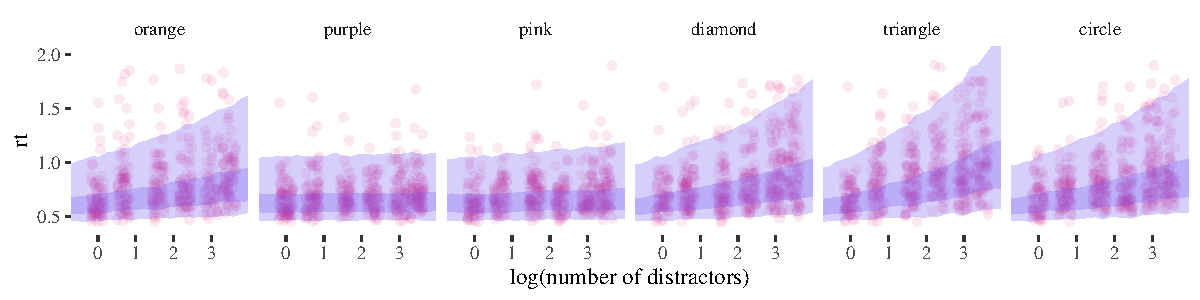
\includegraphics[width=\textwidth]{../plots/sft_ln_model.pdf}
%\end{subfigure}
%\begin{subfigure}
%\centering
%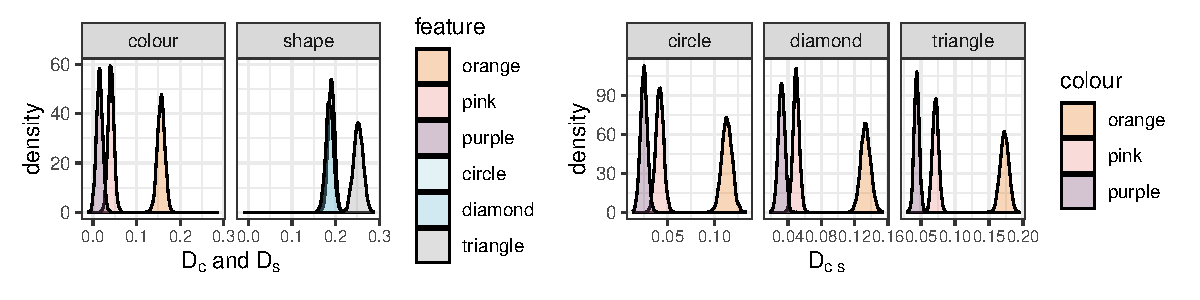
\includegraphics[width=\textwidth]{../plots/Dcs.pdf}
%\end{subfigure}
%\caption{(\textit{top})The shifted-lognormal model fits for the single-feature data. / Data points show a random sample of $10\%$ of the individual trials from our experiment. Shaded region shows the $53\%$ and $97\%$ HPDI for the fixed-effect component of the shifted-lognormal model (loglinear in $N_T$). (\textit{bottom}) Values for $D_c$, $D_s$ and $D_{c,s}$ from the shifted lognormal model. These are comparable to traditional search slopes, except that our model has a log-log relationship between the number of distractors and response times.}
%\label{fig:sftln_sf}
%\end{figure}

\subsection{Hypothesis 2: log-linear effect of $N_T$}

We then used the same methods to verify that using $\log{N_T}$ for the search slope does indeed give a better fit to the data than simply using $N_T$. The results are again conclusive with $\sim100\%$ of the model weight being assigned to the model that is log-linear in $N_T$. 

\subsection{Hypothesis 3: Contrast Model Comparison}

Now that we have confirmed that the shifted-lognormal multilevel model (with a log-linear effect of $N_T$) is indeed the best fit to the data we will extract the search slopes for each feature. These are summarised in Table \ref{tab:new_Dc_Ds}. We can see that we have successfully obtained a range of values for both $D_c$ and $D_s$. As with \cite{buetti2019predicting} we find that the values for $D_s$ are larger than $D_c$ (see Table \ref{tab:reimp_Dc_Ds}), meaning that search slopes for colour features are shallower than shape. 

\begin{table}[h]
\centering
\begin{tabular}{|c|cc||c|cc|} 
\hline
feature & $D_c$ & $95\%$HDCI &feature &$D_s$  &$95\%$HDCI \\
 \hline 
orange & 0.161 &  [0.144 ,  1.110] & triangle  &  0.258  & [0.237  , 0.849]\\
pink  &  0.039 &  [-0.061 , 0.053] & diamond& 0.190 &  [0.174 ,  1.168]\\
purple & 0.019 &  [0.005  , 0.537] & circle & 0.188  & [-0.065 , 0.202]\\
 \hline 
 \end{tabular}
\caption{A summary of the posterior estimates of $D_c$ and $D_s$ values from our Experiment. Note that our values are reported in seconds, in contrast to Table  \ref{tab:reimp_Dc_Ds}, which follows \citep{buetti2019predicting} and reports the slopes in milliseconds.}
\label{tab:new_Dc_Ds}
\end{table}

We now combine the \textit{single-feature} search slopes, $D_c$ and $D_s$, to predict the \textit{double-feature} conditions ($D_{c,s}$) using Equations \ref{eq:bestfeature},  \ref{eq:orthogonalcontrast} and \ref{eq:collinearcontrast} and above. The results are summarised in Figure \ref{fig:new:Dpe}. We find that while the collinear contrast model has the highest $R^2$ (0.922, compared to $R^2=0.883$ for best feature, and $R^2=0.915$ for orthogonal contrast), the orthogonal contrast model is the most accurate, both in terms of mean absolute error (0.165, compared to 0.185 for best feature and 0.271 for collinear) and having a regression slope closest to 1 (0.999 compared to 0.748 and 1.48). Therefore, Hypothesis 3 does not hold: orthogonal contrast rather than collinear contrast offers the best prediction of search slopes in the double-feature condition.  

\begin{figure}[ht]
\centering
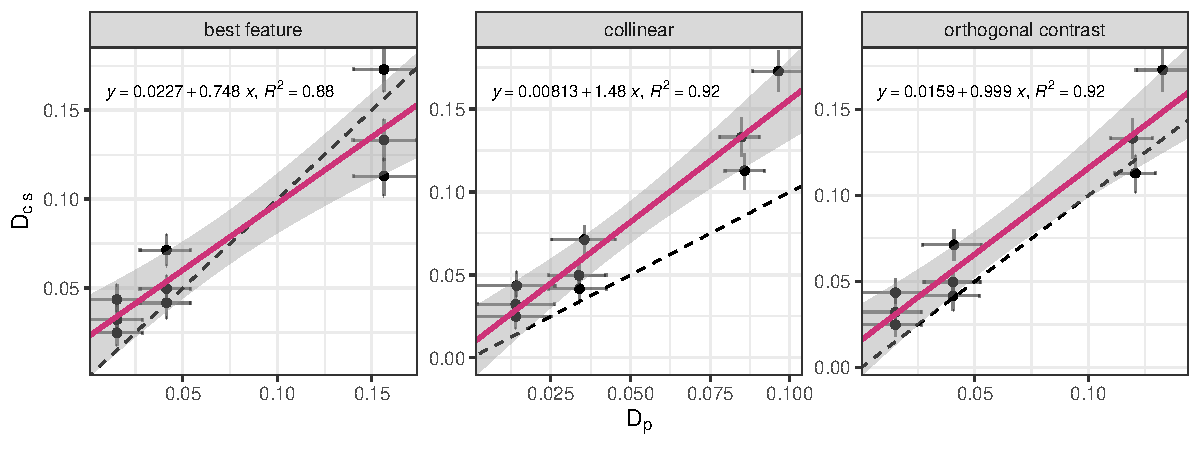
\includegraphics[width=\textwidth]{../plots/Dpe.pdf}
\caption{Predicting $D_{c,s}$ from $D_c$ and $D_s$. The $x$-axis shows our predictions, $D_p$, using the best feature, collinear contrast, and orthogonal contrast models.}
\label{fig:new:Dpe}
\end{figure}

\subsection{Hypothesis 4: Reaction Time Predictions}

Upon reflection, the approach to model comparison we outlined in our registered analysis was limited in a number of ways. Our original plan was to use the posterior predictions from a model trained on the single-feature data to act as a prior for the double-feature data. While we initially thought this would be an elegant approach, there are a large number of parameters that are outside the main focus of this paper yet still require priors (intercepts, group level variance and residual variance). Furthermore, while the methods for estimating $D_{c,s}$ presented above give good predictions in terms of the mean value, it is not clear that the standard deviation for these distributions will be accurate. As such, we have developed a new, simpler method for this final comparison. To maintain full transparency, we present both methods here. 

\subsubsection{Registered Method}

Our final hypothesis concerns how well the different feature combination models perform when predicting reaction times. We find very little difference between the three methods in terms of LOO model weights: 0.294 for best feature, 0.341 for collinear and 0.365 for orthogonal contrast. 

\subsubsection{Updated Method}

Our new method for exploring this hypothesis involves taking $n=1000$ samples of the fixed effects from both the model fitted to the single-feature data and the model fitted to the double-feature data. Each of these samples includes an intercept ($a$), slope ($D$), non-decision time ($\text{ndt}$, and residual variance ($\sigma$). We then take the parameters from the double-feature model, but replace the $D$ values with our predicted $D$ using the single-feature model. We can then calculate:

\begin{itemize}
    \item the predicted mean $\log(rt)$ for each feature and number of distractors. These are then compared to the empirical reaction times and we calculate the absolute error
    \item the log-likelihood of each empirical reaction time given the mean $\log(rt)$, $sigma$ and $\text{ndt}$
\end{itemize}

We can also calculate an upper-bound by carrying out the above process, but without replacing the fitted $D$ with the predicted. This allows us to report relative error and likelihood. As all of the methods under consideration make identical predictions for trials with no distractors, these are omitted from this calculation. Finally, we calculate the mean relative log-likelihood and relative absolute error over the 1000 samples from the original statistical model. 

The results of this procedure are in-line with the registered analysis above with all three methods performing well relative to our baseline (see Table \ref{tab:new_pred_rt}), but little distinction between the three models.

\begin{table}[h]
\centering
\begin{tabular}{c|ccc|ccc} 
\hline
metric & & abs error & &  & loglik  & \\
 \hline
  & lower  & median & upper & lower  & median & upper \\
 
orthogonal & 0.992 & 1.00 & 1.02 & 0.978 & 0.988 & 0.998\\
collinear & 0.990 & 1.01 & 1.03 & 0.968 & 0.977 & 0.985\\ 
best feature  & 1.00 & 1.02 & 1.02 & 0.985 & 0.999 & 1.01\\
 \end{tabular}
\caption{How well can we predict RTs using $D_p$ (collinear, best feature or orthogonal contrast) comped to using $D_e$. A value of 1 means that out estimates of $D$ derived from the single-feature trials does an equally good job at predicting the double-feature trials as using the $D$ fit to the data.}
\label{tab:new_pred_rt}
\end{table}


\section{Planned Explorations}

\subsection{Individual Differences}

We start this exploratory analysis looking at how the $D_c$ and $D_s$ values vary from participant to participant. From Figure \ref{fig:exp_corr} (\textit{left}) we can see that there is considerable variation between observers - in fact, the variation from one observer to the next is often larger than the variation across features. To investigate this further we calculated the correlations between each of the features, by  calculating Pearson's $r$ for each sample from our posterior, which gives us a full posterior distribution for the correlations. We can see in Figure \ref{fig:exp_corr} (\textit{right}) that while both the $D_c$ and $D_s$ are correlated within feature classes ($\sim0.75$), there is no correlation of any of the colour features with any of the shape features. The individual differences for the \textit{double-feature} conditions are much less pronounced - these conditions are easy and the search slopes are quite close to flat (CHECK this!). Hence, the correlations are all much weaker, presumably due to range restriction. 

\begin{figure}[ht]
\centering
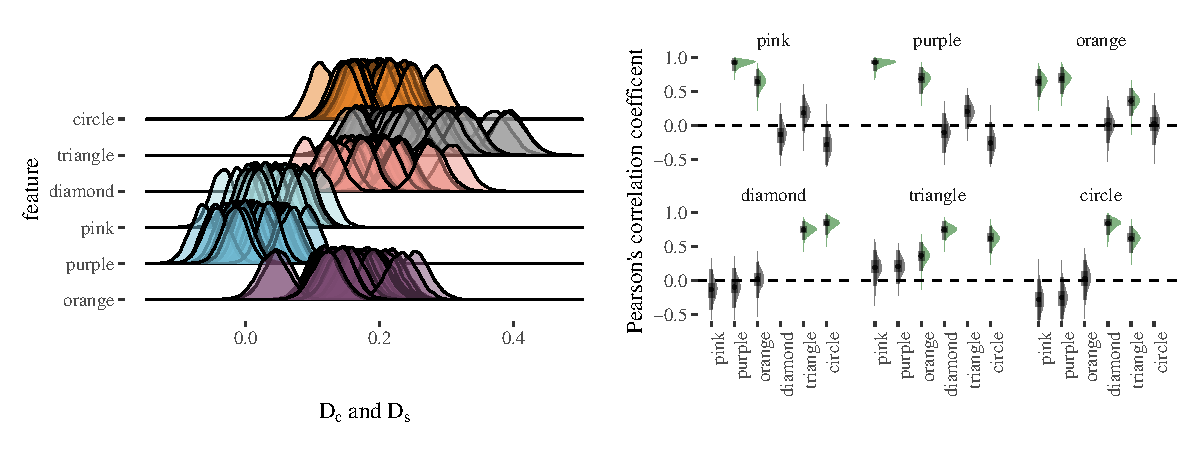
\includegraphics[width=\textwidth]{../plots/single_feature_correlations.pdf}
\caption{Individual differences in $D_c$ and $D_s$. (\textit{left}) Posterior probability distributions for $D_c$ and $D_s$ for each individual. (\textit{right}) Estimated correlations between each of the $D_c$ and $D_s$.}
\label{fig:exp_corr}
\end{figure}

Given these results, it is perhaps unsurprising that our analysis for Hypothesis 4 leads to an inconclusive result for distinguishing between the three contrast combination methods. Perhaps taking these individual differences into account when we predict reaction times will lead to improved power to discriminate between the models. However, before we do so, we will also investigate incorporating information about target eccentricity into the model.

\subsection{Target Eccentricity}

It is well known that there are eccentricity effects in visual search, with reaction times being longer for targets that are further away from fixation \citep{carrasco1995eccentricity}. To investigate this in our dataset, we will use the same methods as above (fitting a multi-level shifted-lognormal model) but now including an additional factor that represents how far the target was from the fixation cross. This is coded as a three-level categorical factor representing which ring contained the target (see stimulus details, above). Allowing for interactions with the \textit{feature} and $\log{N_T}$ increases the number of fixed effect parameters in the model from X to XXX. 

\begin{equation}
y \sim 0 + r + r:f:\log(N_T) + (1|id)
\end{equation}

We experimented with including $r$ in the random effect structure, but this proved difficult to fit. We also had to revise the priors used in our registered analysis, in order to lower the intercept. Full details can be found in the supplementary materials. 

After obtaining a model that passed all convergence checks, we examined the posterior distribution for the effect of \textit{ring}. Figure \ref{fig:ring1} paints an interesting and complex picture in which some features (e.g. some colours, particularly those that are more distinct from the target colour) are clearly leading to `pre-attentive search` in which response times are unaffected by either the number of distractors or target eccentricity. However, shape features seem to be strongly affected by eccentricity, particularly when there are multiple distractors in the stimulus.

\begin{figure}[ht]
\centering
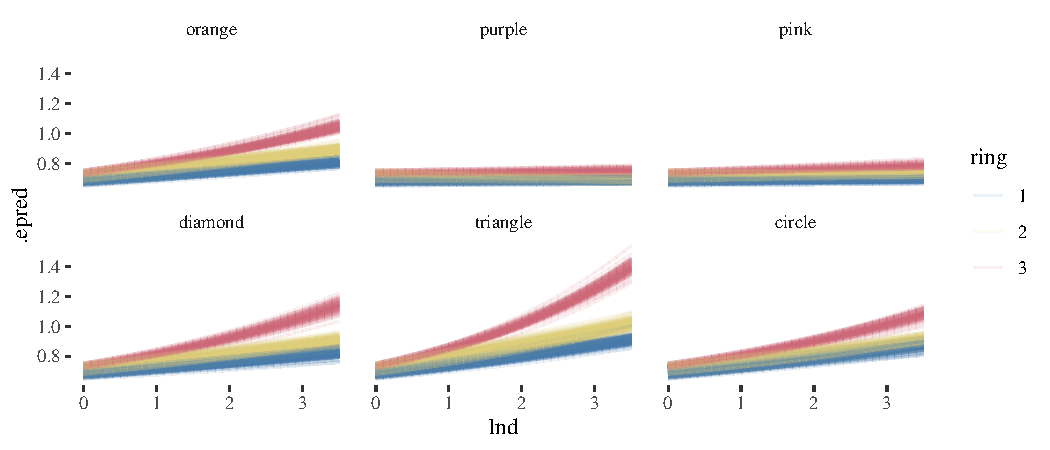
\includegraphics[width=\textwidth]{../plots/ring_single_feature.pdf}
\caption{Fixed effects for predicting the effect of ring, feature and number of distracters on response times. SWITCH TO HPDI PLOT TO BE CONSISTENT WITH WHAT WE USED BEFORE. Shaded regions represent $97\%$ HPDI. We can see that \textit{ring} has an effect on search slopes, and that this effect is more pronounced for some features (i.e., triangles) than others.}
\label{fig:ring1}
\end{figure}

We can now compute our predictions ($D_p$) for $D_{c,s}$ taking the \textit{ring} into account. Doing so leads us to a similar result as before with orthogonal contrast outperforming the best feature and collinear measures in terms of absolute error (0.23 compared to 0.25 (best feature) and 0.34 (collinear)). However, the regression slopes are all relatively similar (0.90 for best feature, 1.16 for collinear and 1.15 for orthogonal contrast - CHECK).

\subsection{Predicting Response Times}

We will now test to see if we can discriminate between the three contrast combination methods when we take target eccentricity (ring) and individual-level slopes into account. We use the same model comparison as before (see Supplementary Materials for full code) and find orthogonal contrast performs best (), closely followed by best feature. 

\subsection{Issues with the Collinear Contrast method}
The collinear contrast method performs very poorly in this test. To explain this, we can look back at Equation \ref{eq:collinearcontrast} and realise that empirical data is not required to reject this hypothesis as a suitable method for predicting search slopes in feature search. This is because when search slopes are close to 0, it is possible that we will observe negative values in the empirical data. Breaking down our data to compute search slopes for each person and each target eccentricity increases the chances of this being observed. Looking at Equation \ref{eq:collinearcontrast} we can see that $D_1 \sim -D_2\Rightarrow 1/D_1 + 1/D_2 \sim 0$. This leads to our estimated $D = \frac{1}{1/D_1 + 1/D_2} >>> D_1, D_2$ which is clearly incorrect. 

\section{General Discussion}

In this paper, we aimed to test the extent to which the results of \cite{buetti2019predicting} replicate and generalise, using a new modelling approach. Our results allow us to confirm our pre-registered hypotheses 1 and 2. Firstly, a shifted-lognormal distribution of response times outperforms normal and lognormal distributions, demonstrating that reaction time data is best modelled by a distribution with an offset (as valid responses begin at around 100ms). Similarly, we confirmed that the number of distractors has a log-linear effect in this model, in line with the predictions of TCS theory. We also replicated other aspects of the original \cite{buetti2019predicting} paper with a different experimental set up, such as the fact that we saw shallower search slopes for colour features compared to shape features.

However, we do not find support for our pre-registered hypotheses 3 and 4. For predicting D for the double-feature conditions, our analyses found that the orthogonal contrast model was favoured over collinear, which is not in line with the registered hypothesis, which predicted that the collinear contrast model would be best (in line with \cite{buetti2019predicting}). Similarly, for hypothesis 4, we found that there was relatively little difference between the three combination methods for prediction of trial-by-trial reaction times. Our exploratory analyses suggest that incorporating additional factors (e.g. individual differences in participant $D_c$ and $D_s$ values, and the eccentricity of the target) allows better discrimination between models, but again suggests that the orthogonal contrast combination method gives the best predictions.

\subsection{Modelling of reaction times}

In much of the literature on visual search (cite some examples), mean reaction times are modelled using a simple linear model $\bar{y} = b N_T + a$. The $b$ coefficients are often referred to as ``search slopes'' and are often treated as measurements of theoretical importance <HOW TO PHRASE PROPOPERLY?>. The results presented above indicate that a shifted-lognormal model that is loglinear in $N_T$ offers a much better fit to the data.

This result isn't particularly novel. For example, \cite{buetti2019predicting} use $\log{N_T}$ when computing their search slopes (also see CITE STUFF). In terms of reaction time distributions, researchers have looked at which distribution offers the best fit to empirical response times in visual search before. For example, \cite{palmer2011shapes} compared ex-Gaussian, ex-Wald, Gamma, and Weibull distributions and found that the distributions with exponential components offer a better fit to the data. Our results are in line with this. However, we opted to use a shifted-lognormal distribution in our analysis above for pragmatic reasons (INSERT NOTE HERE). In most situations we would expect it to be difficult to distinguish between these different distributions. Also see \citep{wolfe2010reaction}. It is also worth mentioning that some more sophisticated approaches make use of drift-diffusion methods (cite some examples) (cite some of the papers outlining why these models can be difficult).  

Despite these previous findings, the use of linear search slopes is still prevalent in the visual search literature (can we find any examples? Do we want to name names?). We recommend that other researches make use of these more sophisticated models when calculating search slopes. Our work shows that these choices of distribution can influence results and conclusions.

\subsection{Discriminating between combination methods}

, despite the fact that the collinear contrast model had the lowest mean error in our pilot data analysis, in line with the findings from the original manuscript. However, all three models have similar predictive weight which means that arguably it is difficult to distinguish which model is best, and that small changes in participant responses might alter the preferred model (and the preferred model may also vary depending upon which metric is considered).

Our interpretation of the null/neutral results for Hypothesis 4 (the prediction of reaction times) is that the differences in predictions from the three contrast combination methods are small relative to the (i) individual differences between participants and (ii) trial-to-trial variability due to target eccentricity.

 
\subsubsection{Individual differences}

INDIVIDUAL DIFFS - While it is not possible to determine whether this pattern is caused by differences in colour v.s. shape features, or by the block structure used in our experiment either way, this is an intriguing result. 

\textit{say something about correlations/. can cite \cite{clarke2020stable}}

\subsubsection{Eccentricity}

\subsection{Lessons learned from our modelling approach}

Do we want to discuss that evaluating these methods on all number of distractors is kinda dumb, and we should really look at only case in which we have a large number of distractors?
Averages vs. individuals? Maybe want some citations here - what are we trying to do with our models?


% Authors must disclose all relationships or interests that 
% could have direct or potential influence or impart bias on 
% the work: 
%
\section*{Conflict of interest}
The authors declare that they have no conflict of interest.

\section*{Acknowledgements}
This work was supported by an Economic and Social Research Council grant (ES/S016120/1) to ADFC and employing AN.

% BibTeX users please use one of
\bibliographystyle{plainnat}    % basic style, author-year citations
%\bibliographystyle{spmpsci}      % mathematics and physical sciences
%\bibliographystyle{spphys}       % APS-like style for physics
\bibliography{sources}   % name your BibTeX data base

\end{document}